% You should title the file with a .tex extension (hw1.tex, for example)
\documentclass[11pt]{article}

\usepackage{amsmath}
\usepackage{amssymb}
\usepackage{fancyhdr}
\usepackage{listings}
\usepackage{color}
\usepackage{graphicx}
\graphicspath{ {images/} }
\usepackage{hyperref}
\usepackage{mathtools}

\definecolor{dkgreen}{rgb}{0,0.6,0}
\definecolor{gray}{rgb}{0.5,0.5,0.5}
\definecolor{mauve}{rgb}{0.58,0,0.82}

\lstset{frame=tb,
  language=Java,
  aboveskip=3mm,
  belowskip=3mm,
  showstringspaces=false,
  columns=flexible,
  basicstyle={\small\ttfamily},
  numbers=none,
  numberstyle=\tiny\color{gray},
  keywordstyle=\color{blue},
  commentstyle=\color{dkgreen},
  stringstyle=\color{mauve},
  breaklines=true,
  breakatwhitespace=true,
  tabsize=3
}

\oddsidemargin0cm
\topmargin-2cm     %I recommend adding these three lines to increase the 
\textwidth16.5cm   %amount of usable space on the page (and save trees)
\textheight23.5cm  

\newcommand{\question}[2] {\vspace{.25in} \hrule\vspace{0.5em}
\noindent{\bf #1: #2} \vspace{0.5em}
\hrule \vspace{.10in}}
\renewcommand{\part}[1] {\vspace{.10in} {\bf (#1)}}

\newcommand{\myname}{Chang-Hyun Mungai}
\newcommand{\myhwnum}{Creation Notes}

\setlength{\parindent}{0pt}
\setlength{\parskip}{5pt plus 1pt}
 
\pagestyle{fancyplain}
\lhead{\fancyplain{}{\textbf{\myhwnum}}}      % Note the different brackets!

\begin{document}

\medskip                        % Skip a "medium" amount of space
                                % (latex determines what medium is)
                                % Also try: \bigskip, \littleskip

\thispagestyle{plain}
\begin{center}                  % Center the following lines
{\Large Creation} \\
\end{center}

\question{General}

\begin{itemize}
   \item deal with object creation mechanisms, trying to create objects in a manner suitable to the situation
   \item These design patterns are all about class instantiation 
   \item This pattern can be further divided into class   \item creation patterns and object   \item creational patterns
   \item While class   \item creation patterns use inheritance effectively in the instantiation process, object   \item creation patterns use delegation effectively to get the job done
   \item The creational patterns aim to separate a system from how its objects are created, composed, and represented
   \item They increase the system's flexibility in terms of the what, who, how, and when of object creation
\end{itemize}

\question{Abstract Factory}

\begin{itemize}
   \item Definition/Use

   \begin{itemize}
     \item provides an interface for creating related or dependent objects without specifying the objects' concrete classes
     \item provide an interface for creating families of related or dependent objects without specifying their concrete classes
     \item encapsulates "new" ex: new product()
     \item determines concrete type but returns abstract pointer

     \begin{itemize}
       \item client code has no knowledge and isn't burdened by concrete type
       \item adding new concrete types done by modifying client code to use different factory (1 line)
     \end{itemize}

     \item can determine concrete type from config file for example
   \end{itemize}


   \item Structure

   \begin{itemize}
    \item 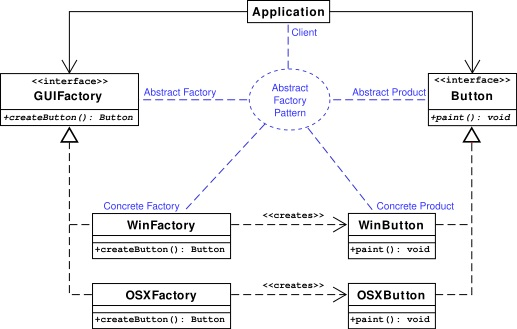
\includegraphics{abstract_factory_class_diagram}
   \end{itemize}
\end{itemize}

\question{Builder}

\begin{itemize}
   \item Definition/Use

   \begin{itemize}
     \item separates the construction of a complex object from its representation so that the same construction process can create different representations
     \item builder pattern is useful to avoid a huge list of constructors for a class
     \item an application needs to create the elements of a complex aggregate
     \item use builder to store parameters and then use that builder in constructor
     \item separate the construction of a complex object from its representation so same construction can create different representations
   \end{itemize}

   \item Structure

   \begin{itemize}
     \item 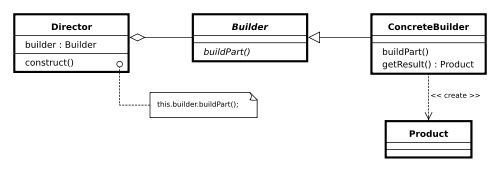
\includegraphics{builder_uml_class_diagram}
     \item 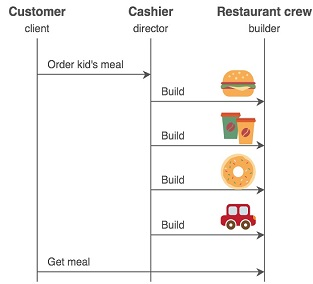
\includegraphics{builder_example}
   \end{itemize}

   \item Example

   \begin{itemize}
     \item StringBuffer and StringBuilder
   \end{itemize}

   \item Notes

   \begin{itemize}
     \item put the builder term in the name of the builder class to indicate the use of the pattern to the other developers
     \item if the target class contains flat data, your builder class can be constructed as a Composite that implements the Interpreter pattern
   \end{itemize}

\end{itemize}

\question{Factory Method}

\begin{itemize}
   \item Definition/Use

   \begin{itemize}
     \item allows a class to defer instantiation to subclasses
     \item new operator considered harmful
     \item define an interface for creating an object, but let subclasses decide which class to instantiate
     \item provide a way for users to retrieve an instance with a known compile-time type, but whose runtime type may actually be different
     \item an increasingly popular definition of factory method is: a static method of a class that returns an object of that class' type

     \begin{itemize}
       \item unlike a constructor, the actual object it returns might be an instance of a subclass
     \end{itemize}

   \end{itemize}

   \item Structure

   \begin{itemize}
     \item 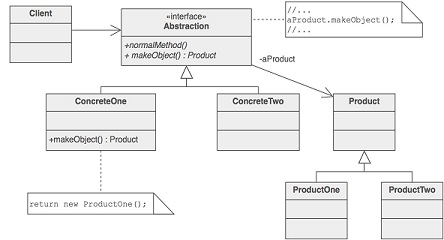
\includegraphics{factory_method_example}
   \end{itemize}

   \item Example

   \begin{itemize}
     \item a factory method that is supposed to return an instance of the class Foo may return an instance of the class Foo, or an instance of the class Bar, so long as Bar inherits from Foo
     \item 

\begin{lstlisting}
Color.make_RGB_color(float red, float green, float blue)
Color.make_HSB_color(float hue, float saturation, float brightness)
\end{lstlisting}

     \item

\begin{lstlisting}
 Letter.getLetter(char) if vowel return Vowel(char) else Consonant(char) (vowel, consonant extend letter)
\end{lstlisting}
   \end{itemize}

   \item Notes

   \begin{itemize}
     \item consider making all constructors private or protected
   \end{itemize}

\end{itemize}

\question{Prototype}

\begin{itemize}
   \item Definition/Use

   \begin{itemize}
     \item specifies the kind of object to create using a prototypical instance, and creates new objects by cloning this prototype
     \item when the type of objects to create is determined by a prototypical instance, which is cloned to produce new objects
     \item application "hard wires" the class of object to create in each "new" expression
   \end{itemize}

   \item Structure

   \begin{itemize}
     \item 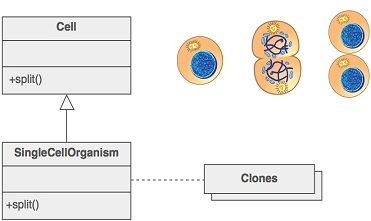
\includegraphics{prototype_example}
     \item 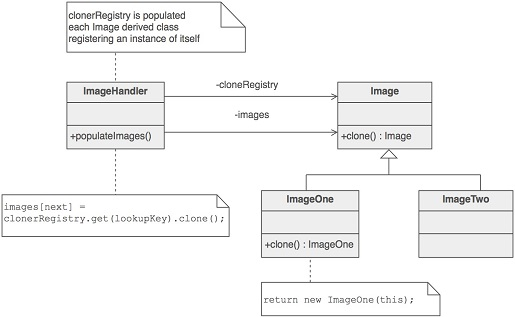
\includegraphics{prototype_structure}
     \item 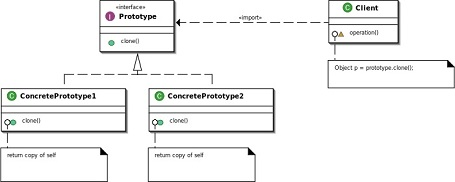
\includegraphics{prototype_uml_structure}
   \end{itemize}

   \item Notes

   \begin{itemize}
     \item add clone() method
     \item add registry
     \item put the prototype term in the name of the prototype classes to indicate the use of the pattern to the other developers
   \end{itemize}

\end{itemize}

\question{Singleton}

\begin{itemize}
   \item Definition/Use

   \begin{itemize}
     \item ensures that a class only has one instance, and provides a global point of access to it
     \item ensure a class has only one instance, and provide a global point of access to it
   \end{itemize}

   \item Structure

   \begin{itemize}
     \item 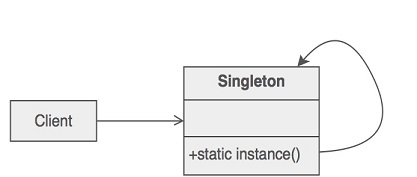
\includegraphics{singleton_structure}
   \end{itemize}

   \item Notes

   \begin{itemize}
     \item make instantiation(private ThisSingleton(){}) private aka define all constructors to be protected or private
     \item name the method getInstance() to indicate the use of the pattern to the other developers
     \item define a private static attribute in the "single instance" class
   \end{itemize}

\end{itemize}
 
\question{Comparison}

\begin{itemize}
   \item abstract Factory classes are often implemented with Factory Methods, but they can be implemented using Prototype
   \item factory method: creation through inheritance, prototype: creation through delegation
\end{itemize}

\end{document}

